\documentclass[a4paper]{article}

\usepackage{latexml}
\usepackage[T1, T5]{fontenc}
\usepackage[utf8]{inputenc}
\usepackage{amsmath}
\usepackage{amsthm}
\usepackage{amssymb}
\usepackage{tikz}
\usetikzlibrary{shapes}
\usepackage[american,vietnamese]{babel}
\usepackage[unicode]{hyperref}
\usepackage{algorithm, algpseudocode}
\usepackage{graphicx}
\usepackage{tabularx}
\newcolumntype{Y}{>{\centering\arraybackslash}X} % center align in X column (using Y instead of X)
\usepackage{multirow}
\usepackage{array}
\usepackage{listings}
\usepackage{color}

\usepackage[sort&compress,numbers,square]{natbib}

\definecolor{mygreen}{rgb}{0,0.6,0}
\definecolor{mygray}{rgb}{0.5,0.5,0.5}
\definecolor{mymauve}{rgb}{0.58,0,0.82}
\definecolor{mybackground}{rgb}{0.83,0.89,0.88}
\definecolor{darkgray}{rgb}{0.66, 0.66, 0.66}
\definecolor{x11gray}{rgb}{0.75, 0.75, 0.75}

\lstset{ 
  backgroundcolor=\color{white},   % choose the background color; you must add \usepackage{color} or \usepackage{xcolor}; should come as last argument
  basicstyle=\ttfamily\small,        % the size of the fonts that are used for the code
  breakatwhitespace=false,         % sets if automatic breaks should only happen at whitespace
  breaklines=true,                 % sets automatic line breaking
  captionpos=b,                    % sets the caption-position to bottom
  commentstyle=\color{mygray},    % comment style
  deletekeywords={...},            % if you want to delete keywords from the given language
  escapeinside={\%*}{*)},          % if you want to add LaTeX within your code
  extendedchars=true,              % lets you use non-ASCII characters; for 8-bits encodings only, does not work with UTF-8
  frame=single,	                   % adds a frame around the code
  keepspaces=true,                 % keeps spaces in text, useful for keeping indentation of code (possibly needs columns=flexible)
  keywordstyle=\color{blue},       % keyword style
%  language=Octave,                 % the language of the code
  morekeywords={*,...},            % if you want to add more keywords to the set
  numbers=left,                    % where to put the line-numbers; possible values are (none, left, right)
  numbersep=5pt,                   % how far the line-numbers are from the code
  numberstyle=\small\color{black}, % the style that is used for the line-numbers
  rulecolor=\color{black},         % if not set, the frame-color may be changed on line-breaks within not-black text (e.g. comments (green here))
  showspaces=false,                % show spaces everywhere adding particular underscores; it overrides 'showstringspaces'
  showstringspaces=false,          % underline spaces within strings only
  showtabs=false,                  % show tabs within strings adding particular underscores
  stepnumber=1,                    % the step between two line-numbers. If it's 1, each line will be numbered
  stringstyle=\color{mymauve},     % string literal style
  tabsize=2,	                   % sets default tabsize to 2 spaces
  title=\lstname                   % show the filename of files included with \lstinputlisting; also try caption instead of title
}

\usepackage{xcolor}

% Solarized colors
%\definecolor{sbase03}{HTML}{002B36}
%\definecolor{sbase02}{HTML}{073642}
%\definecolor{sbase01}{HTML}{586E75}
%\definecolor{sbase00}{HTML}{657B83}
%\definecolor{sbase0}{HTML}{839496}
%\definecolor{sbase1}{HTML}{93A1A1}
%\definecolor{sbase2}{HTML}{EEE8D5}
%\definecolor{sbase3}{HTML}{FDF6E3}
%\definecolor{syellow}{HTML}{B58900}
%\definecolor{sorange}{HTML}{CB4B16}
%\definecolor{sred}{HTML}{DC322F}
%\definecolor{smagenta}{HTML}{D33682}
%\definecolor{sviolet}{HTML}{6C71C4}
%\definecolor{sblue}{HTML}{268BD2}
%\definecolor{scyan}{HTML}{2AA198}
%\definecolor{sgreen}{HTML}{859900}
%
%\lstset{ % Solarized-Dark
%    % How/what to match
%    sensitive=true,
%    % Border (above and below)
%    frame=lines,
%    % Extra margin on line (align with paragraph)
%    xleftmargin=\parindent,
%    % Put extra space under caption
%    belowcaptionskip=1\baselineskip,
%    % Colors
%    backgroundcolor=\color{sbase03},
%    basicstyle=\color{sbase00}\ttfamily,
%    keywordstyle=\color{scyan},
%    commentstyle=\color{sbase1},
%    stringstyle=\color{sblue},
%    numberstyle=\color{sviolet},
%    identifierstyle=\color{sbase00},
%    %identifierstyle=
%    % Break long lines into multiple lines?
%    breaklines=true,
%    % Show a character for spaces?
%    showstringspaces=false,
%    tabsize=2
%}

%\lstset{ % Solarized-Light
%    % How/what to match
%    sensitive=true,
%    % Border (above and below)
%    frame=lines,
%    % Extra margin on line (align with paragraph)
%    xleftmargin=\parindent,
%    % Put extra space under caption
%    belowcaptionskip=1\baselineskip,
%    % Colors
%    backgroundcolor=\color{sbase3},
%    basicstyle=\color{sbase00}\ttfamily,
%    keywordstyle=\color{scyan},
%    commentstyle=\color{sbase1},
%    stringstyle=\color{sblue},
%    numberstyle=\color{sviolet},
%    identifierstyle=\color{sbase00},
%    % Break long lines into multiple lines?
%    breaklines=true,
%    % Show a character for spaces?
%    showstringspaces=false,
%    tabsize=2
%}

\newtheorem{theorem}{Theorem}[section]
\newtheorem{lemma}[theorem]{Lemma}

\theoremstyle{definition}
\newtheorem{definition}[theorem]{Definition}
\newtheorem{example}[theorem]{Example}
\newtheorem{exercise}[theorem]{Exercise}

\theoremstyle{remark}
\newtheorem{remark}[theorem]{Remark}

\numberwithin{equation}{section}

\hypersetup{
	pdfauthor={Duc A. Hoang},
	pdftitle={A LaTeXML Demo},
	pdfsubject={A LaTeXML Demo},
	pdfkeywords={latexml, demo, html, tex},
	pdfproducer={LaTeX},
	pdfcreator={pdflatex}
}

\iflatexml
% no title and author in Jekyll posts
\title{}
\author{}
\else
\title{A LaTeXML Demo}
\author{Duc A. Hoang}
\fi

\begin{document}

\nocite{*}

\selectlanguage{american}

\maketitle

\begin{abstract}
This document is a test to see how things look like when combining HTML files generated with LaTeXML and Jekyll posts.
\iflatexml 
\href{https://hackmd.io/%40UoL-IWG/latexml}{This page} 
\else 
\href{https://hackmd.io/\%40UoL-IWG/latexml}{This page} 
\fi 
contains a nice overview on how to use LaTeXML.
Other versions of this document are available:
\begin{itemize}
	\iflatexml
	\item \href{https://hoanganhduc.github.io/misc/a-latexml-demo/main.pdf}{PDF}.
	\else
	\item \href{https://hoanganhduc.github.io/misc/a-latexml-demo/}{HTML}.
	\fi
	\item \href{https://hoanganhduc.github.io/misc/a-latexml-demo/main.zip}{TeX source}.
\end{itemize}
\end{abstract}

\tableofcontents

\section{Math formulas}

Unordered list

\begin{itemize}
\item Inline formula: $E = mc^2$.
\item Another formula: The equation $ax^2 + bx + c = 0$ has at most two roots.
\end{itemize}

Ordered list

\begin{enumerate}
\item Element 1
\item Element 2
\item Element 3
\end{enumerate}

Equation

\begin{equation}
E = mc^2
\end{equation}

\[
	\sqrt[3]{x^2 + 4x + 4} = ?
\]

\section{Theorems, Lemmas, etc}

\begin{theorem}[Basic Theorem]\label{thrm:1}
We always have $\mathcal{A} = \dots$ and $\mathbb{N} \subseteq \mathbb{Z}$
\end{theorem}

\begin{proof}
It is well-known that ...
\end{proof}

\begin{exercise}
In this exercise, we apply Theorem~\ref{thrm:1} to ...
\end{exercise}

\section{Algorithm}

Here is an example of an algorithm.

\begin{algorithm}[!ht]
\caption{An example algorithm}
\label{alg:1}
\begin{flushleft}
\textbf{Input:} The inputs are ...\\
\textbf{Output:} The outputs are ...
\end{flushleft}
\begin{algorithmic}[1]
\State A statement
\If{The above statement is true}
	\State Do something
\Else
	\State Do nothing
\EndIf
\State \Return something
\end{algorithmic}
\end{algorithm}

Algorithm~\ref{alg:1} computes ...

\section{Cross references}

As in Algorithm~\ref{alg:1}, we have ...

\subsection{Test 1 of subsection}

This is an illustration of a subsection.
This is an illustration of a subsection.
This is an illustration of a subsection.
This is an illustration of a subsection.
This is an illustration of a subsection.

\subsection{Test 2 of subsection and paragraph}

In this section, we will ...
This is an illustration of a subsection.
This is an illustration of a subsection.
This is an illustration of a subsection.

\paragraph{Test paragraph} This is an illustration of a paragraph. This is an illustration of a paragraph. This is an illustration of a paragraph.

\section{Figure}

A figure

\begin{figure}[!ht]
\centering
\begin{tikzpicture}
	\node[circle, very thick, draw=red, fill=yellow] {\textcolor{black}{A circle $C$}};
\end{tikzpicture}
\caption{A figure}
\end{figure}

Another figure taken from the sample \texttt{llncs} class.

\begin{figure}[!ht]
	\centering
	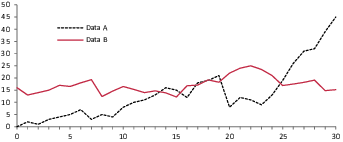
\includegraphics[width=0.7\textwidth]{fig1}
	\caption{A figure from \texttt{llncs} included with \texttt{\textbackslash includegraphics}.}
\end{figure}

\section{Tables}

\begin{table}[!ht]
\begin{tabularx}{\textwidth}{|X|X|}
\hline
Number & Description\\
\hline
1 & One \\
2 & Two \\
3 & Three \\
\hline
\end{tabularx}
\caption{A table.}
\end{table}

\begin{table}[!ht]
\begin{tabularx}{\textwidth}{|Y|Y|Y|Y|}
\hline
\multirow{2}{*}{multi-row} & 1 & 2 & 3 \\
\cline{2-4}
 & 4 & 5 & 6\\
\hline
\multicolumn{3}{|c|}{multi-column} & 7\\
\hline
\end{tabularx}
\caption{A table with multi-row and multi-column.}
\end{table}

\begin{table}[!ht]
\begin{tabularx}{\textwidth}{|r||r@{--}l|X|}
	\hline
	\multicolumn{4}{|c|}{GG\&A Hoofed Stock}
	\\ \hline\hline
	&\multicolumn{2}{c|}{Price}& \\ \cline{2-3}
	\multicolumn{1}{|c||}{Year}
	& \multicolumn{1}{r@{\,\vline\,}}{low}
	& high & \multicolumn{1}{c|}{Comments}
	\\ \hline
	1971 &  97 & 245 & Bad year.\\ \hline
	72 & 245 & 245 & Light trading due to a heavy winter. \\ \hline
	73 & 245 & 2001 & No gnus was very good gnus this year. \\ \hline
\end{tabularx}
\caption{An example from \href{https://dlmf.nist.gov/LaTeXML/examples.html}{LaTeXML Examples Page}.}
\end{table}

\section{Source Code}

Using \verb+verbatim+ environment.

\begin{verbatim}
\begin{table}[!ht]
\begin{tabularx}{\textwidth}{|X|X|}
\hline
Number & Description\\
\hline
1 & One \\
2 & Two \\
3 & Three \\
\hline
\end{tabularx}
\caption{A table.}
\end{table}
\end{verbatim}

Using \verb+listing+ package.

\begin{lstlisting}[language=Python, caption=Python example]
import numpy as np
 
def incmatrix(genl1,genl2):
    m = len(genl1)
    n = len(genl2)
    M = None #to become the incidence matrix
    VT = np.zeros((n*m,1), int)  #dummy variable
 
    #compute the bitwise xor matrix
    M1 = bitxormatrix(genl1)
    M2 = np.triu(bitxormatrix(genl2),1) 
 
    for i in range(m-1):
        for j in range(i+1, m):
            [r,c] = np.where(M2 == M1[i,j])
            for k in range(len(r)):
                VT[(i)*n + r[k]] = 1;
                VT[(i)*n + c[k]] = 1;
                VT[(j)*n + r[k]] = 1;
                VT[(j)*n + c[k]] = 1;
 
                if M is None:
                    M = np.copy(VT)
                else:
                    M = np.concatenate((M, VT), 1)
 
                VT = np.zeros((n*m,1), int)
 
    return M
\end{lstlisting}

\section{References and Citation}

See~\cite{article1}, or~\cite{article2}, or~\cite{article3}.

\bibliographystyle{plainnat}
\bibliography{./refs}

\end{document}
